\origpage{52}{ROBERTSON AND SEYMOUR}
{\centering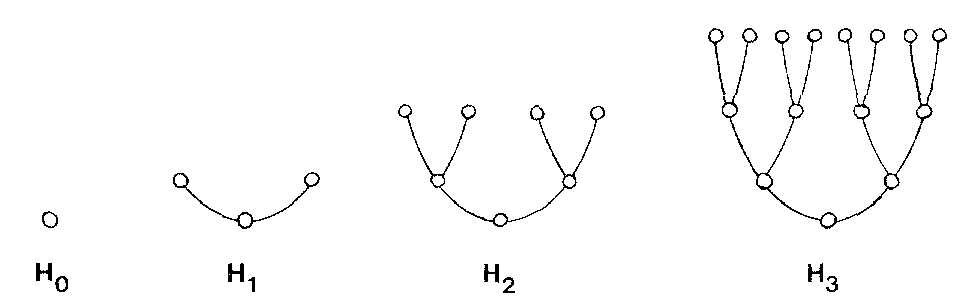
\includegraphics[width=235bp]{figures/fig2}\par
\vspace{12pt}{\small\textsc{Figure} 2}\par}
\stmt
(3.4). \textit{For any odd $\lambda\ge 1$, the $(2^{(\lambda+3)/2}-1)$-grid has a minor isomorphic
to $\mathbf{Y}_\lambda$.}
\stmt
This follows from (3.2) and (3.3).
\stmt
(3.5). \textit{For odd $\lambda\ge 1$, let} $\theta=\max(6, 2^{(\lambda+3)/2})$. \textit{For any graph $G$, if $G$ has
no minor isomorphic to $\mathbf{Y}_\lambda$, then $G\in\mathscr{F}_\theta$.}
\stmt
This follows from (3.4).

Thus to study the graphs with no minor isomorphic to $\mathbf{Y}_\lambda$, we can confine
ourselves to $\mathscr{F}_\theta$, and hence we can apply the results of Section 2.

A \textit{rooted} graph is a graph with one vertex distinguished, called the \textit{root}.
We denote the root of $G$ by $\rho(G)$.

If $G_1, G_2$ are rooted graphs we say that $G_2$ has a \textit{rooted minor isomorphic
to} $G_1$ if for each vertex $v$ of $G_1$ there is a subset $Y(v)$ of the vertices of $G_2$,
satisfying conditions (M1)--(M4):
\stmt
\hspace*{12pt}(M1)\quad\textit{For distinct $v, v'\in V(G_1)$, $Y(v)\cap Y(v')=\varnothing$.}

\hspace*{12pt}(M2)\quad\textit{For each $v\in V(G_1)$, $G_2\,|\,Y(v)$ is connected.}

\hspace*{12pt}(M3)\quad\textit{There is an injection $f\colon E(G_1)\to E(G_2)$ such that for every edge}

{\centering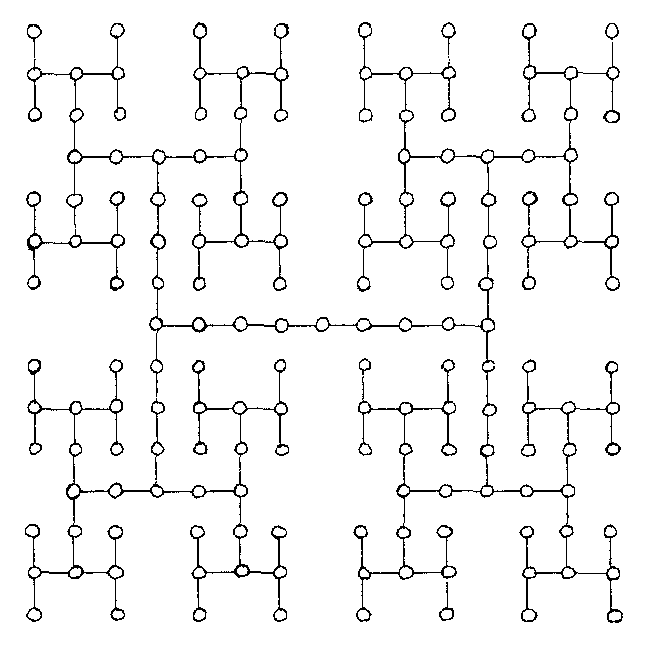
\includegraphics[width=156bp]{figures/fig3}\par
\vspace{12pt}{\small\textsc{Figure} 3}\par}
